\documentclass[12pt]{article}
\usepackage{amsmath}
\usepackage{graphicx}

\title{Report for Auto Control Lab1 and 2}
\date{2020/9/15}
\author{Jacky Yeh 4107064003}

\begin{document}
\begin{titlepage}

\maketitle
\end{titlepage}


\section{Introduction}
This is the first Experiment of Auto Control Lab where TAs taught us some basic concepts and usages in MATLAB for us to better understand the plotting and some basic functions for future learnings.\\

\section{LAB1}
\subsection{Basic usages of plotting functions and matrices}
Objective:To perform basic operations on matrix and plotting graph.\\
These are the stated Homework problems\\
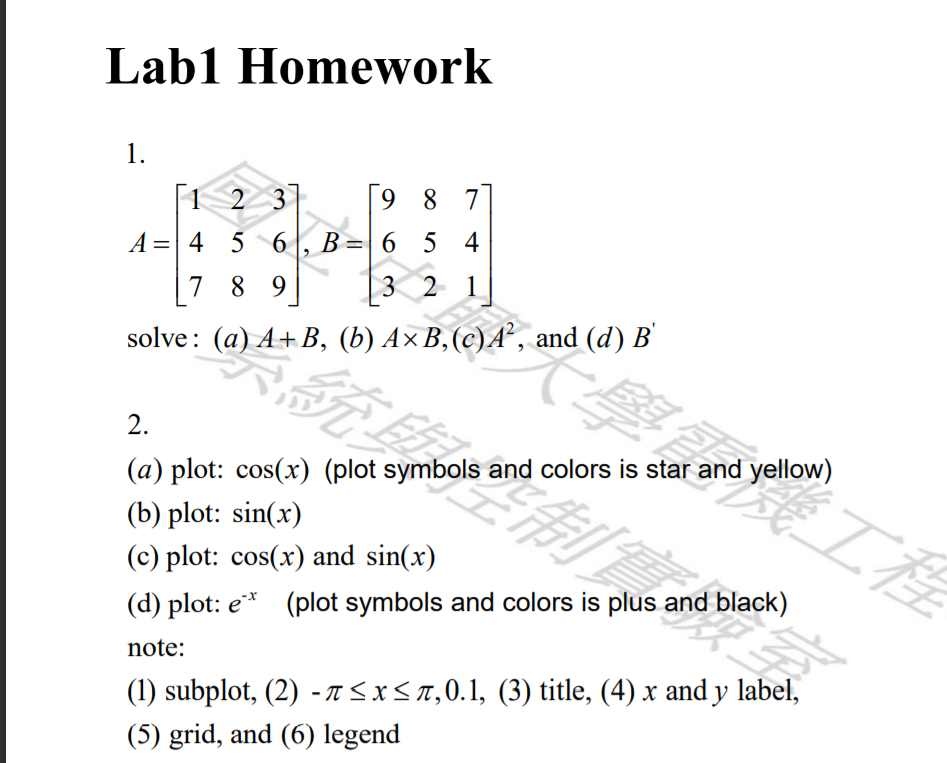
\includegraphics[scale=0.7]{HW first week 9_15 lab/Lab1/Lab1_4.png} \\

\subsection{MATLAB CODE FOR LAB1}
In order to perform the tasks, Matlab codes are needed.The following is the code\\

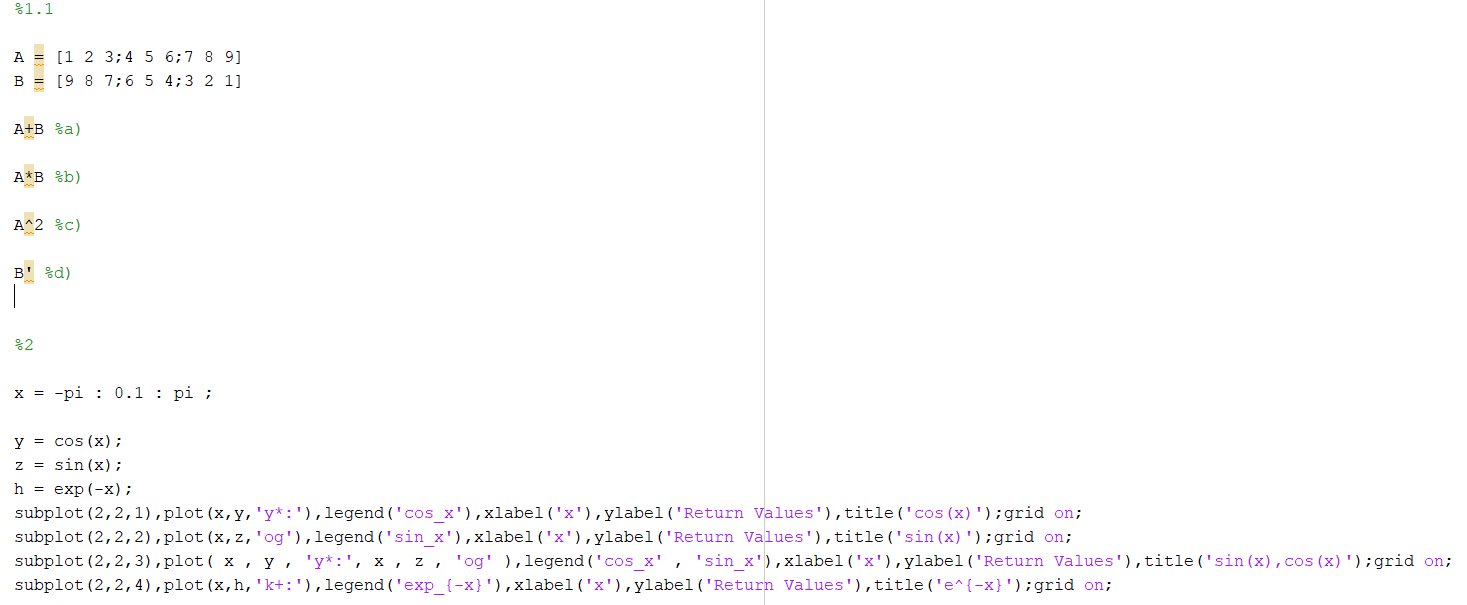
\includegraphics[scale=0.5]{HW first week 9_15 lab/Lab1/Lab1_3.png}\\
\\
The results in this are for the arithmetic operations on matrix A and B\\

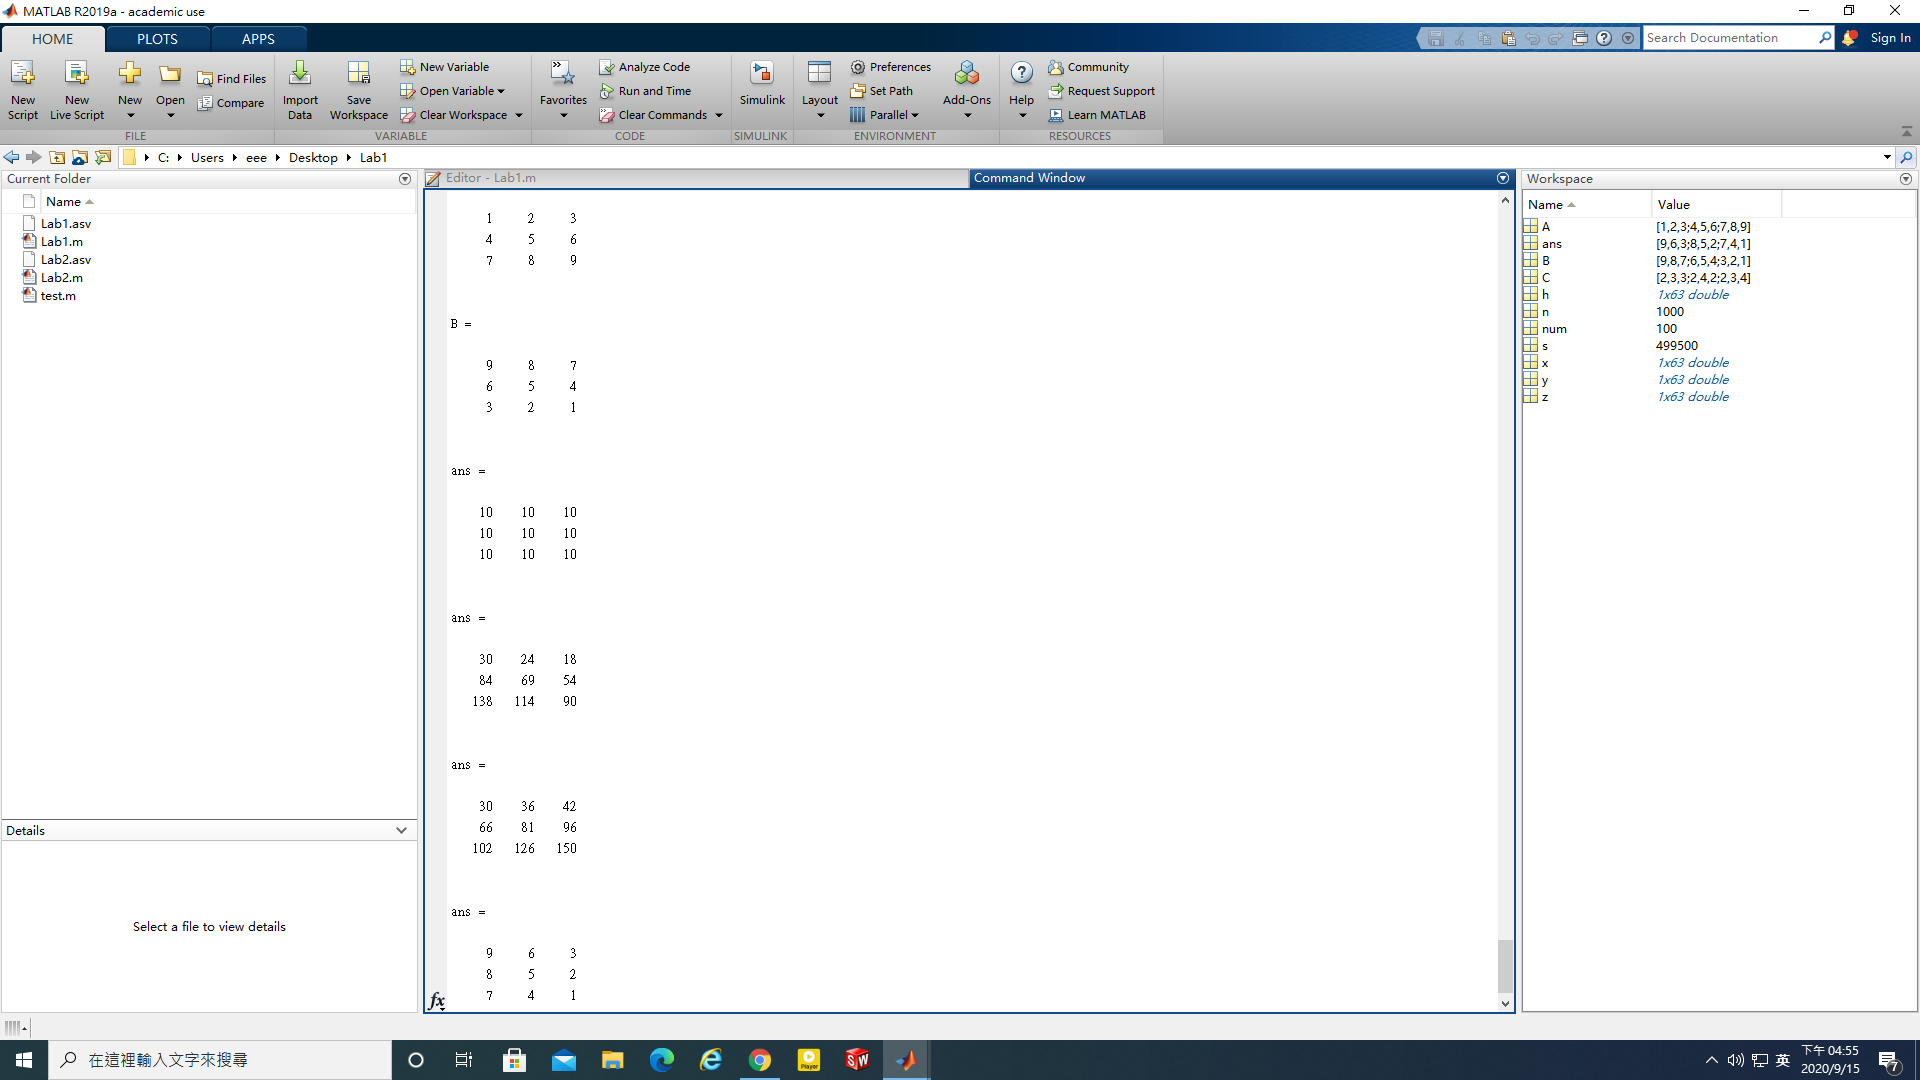
\includegraphics[scale=0.3]{HW first week 9_15 lab/Lab1/Lab1.png}\\

The results in this are the subplots for $cos(x)$,$sin(x)$ and $e^{-x}$ with a 
range from $-\pi \sim \pi$ with titles,grids and legends on\\

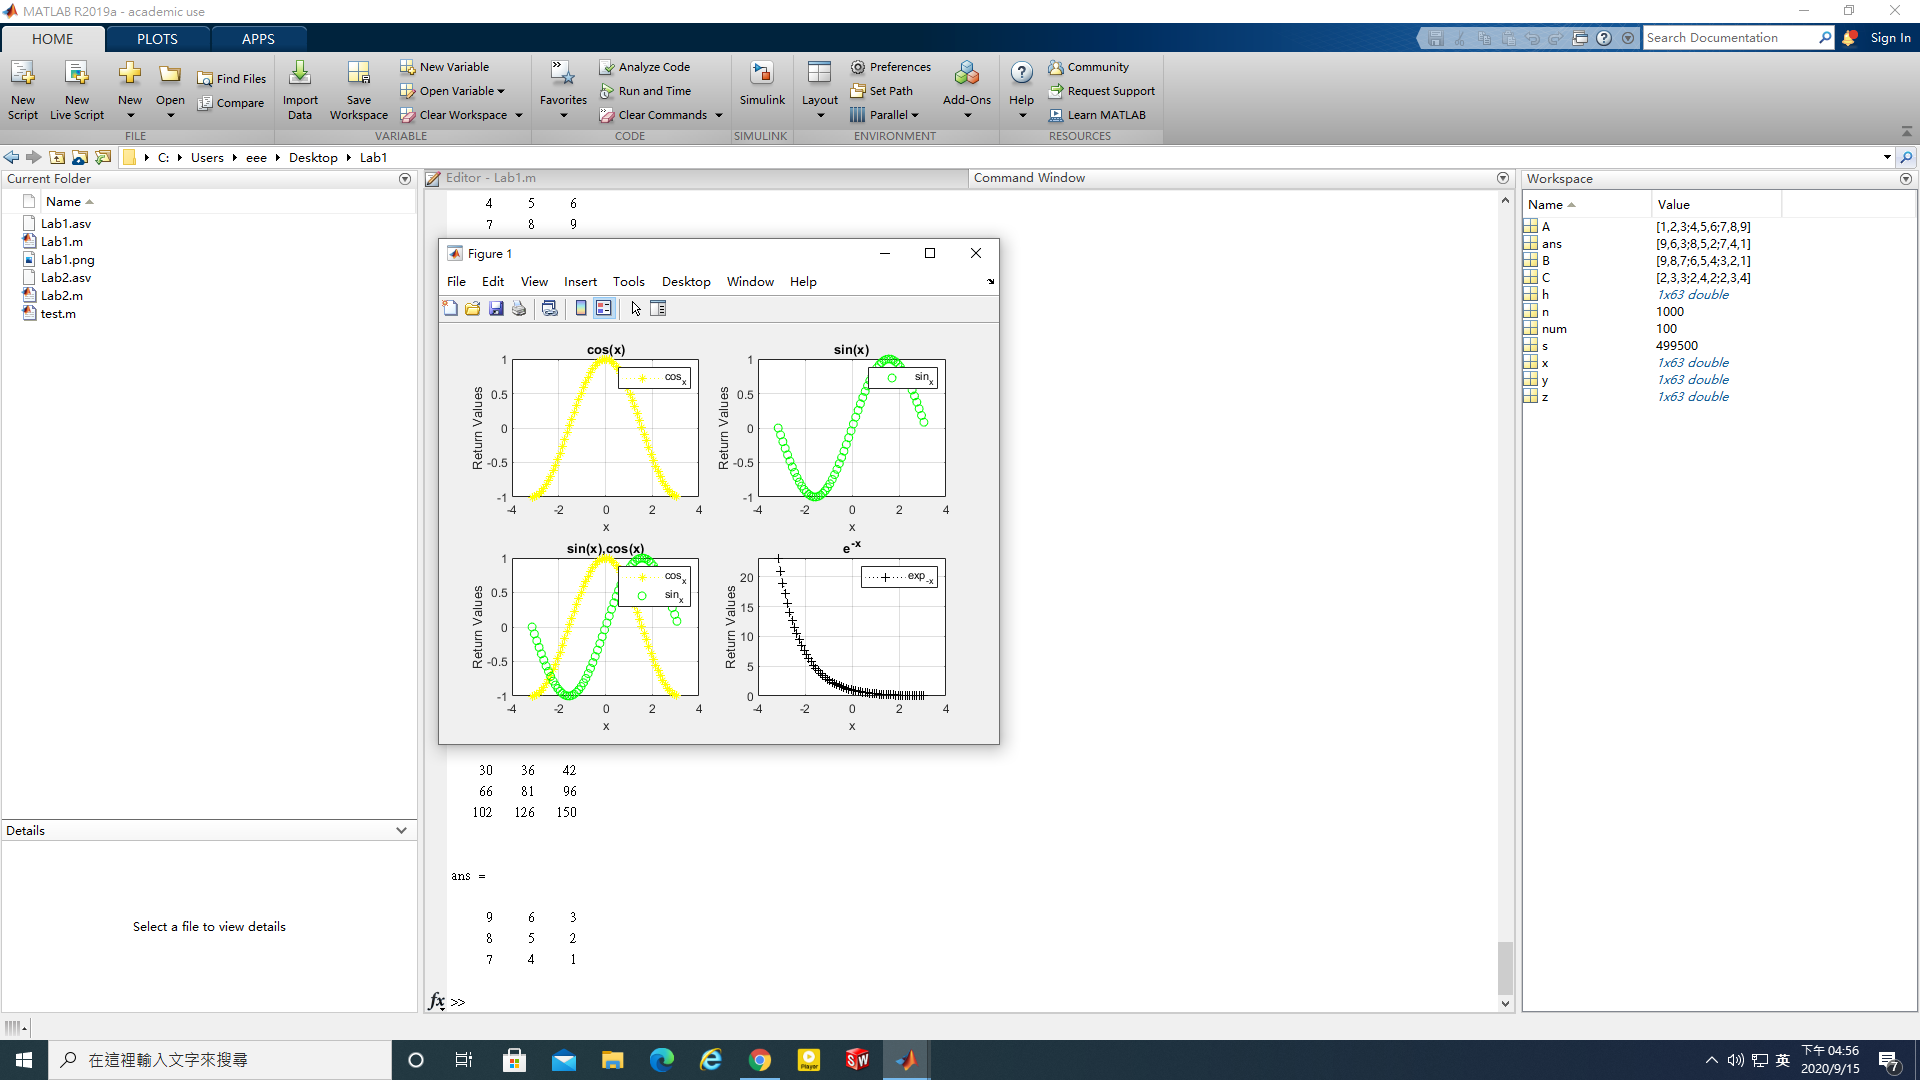
\includegraphics[scale=0.3]{HW first week 9_15 lab/Lab1/Lab1_2.png}\\
 
\cleardoublepage
\section{LAB2}
\subsection{Basic usages of for,while and switch and matrix arithmetic}
Objective:To perform basic functions on matrices and basic usages of iterative functions such as while, for and statement functions such as switch, if\\

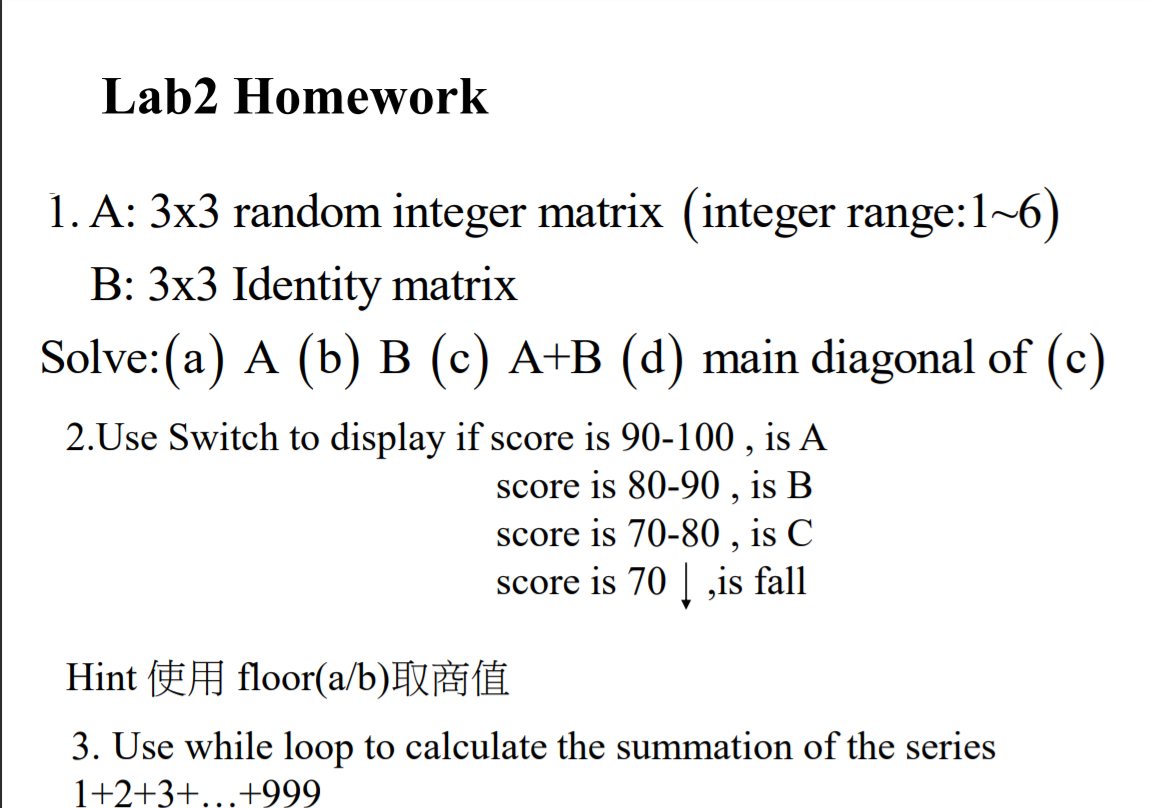
\includegraphics[scale=0.4]{HW first week 9_15 lab/Lab2/Lab2_1.png}

\subsection{Matlab Code for Lab2}
The codes which perform the tasks are stated below\\ 
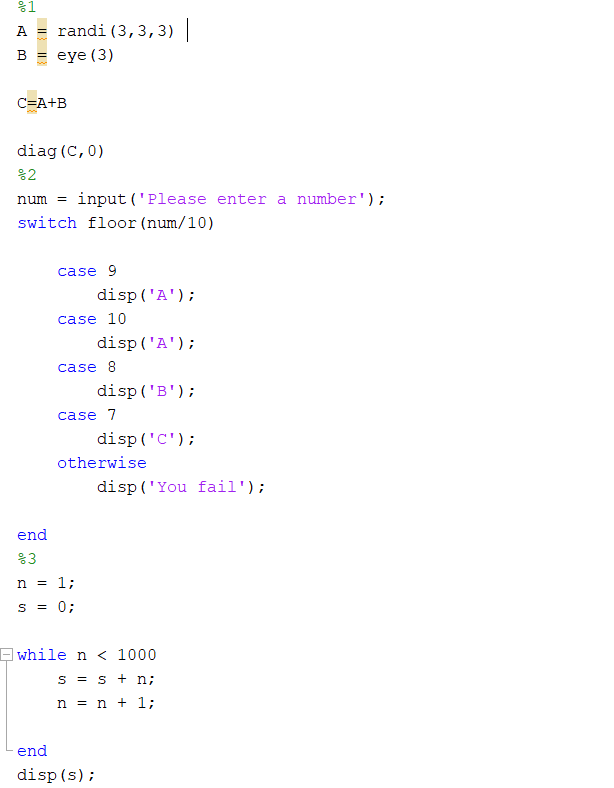
\includegraphics[scale=0.4]{HW first week 9_15 lab/Lab2/Lab2_code.png} \\
The computed results are shown below\\
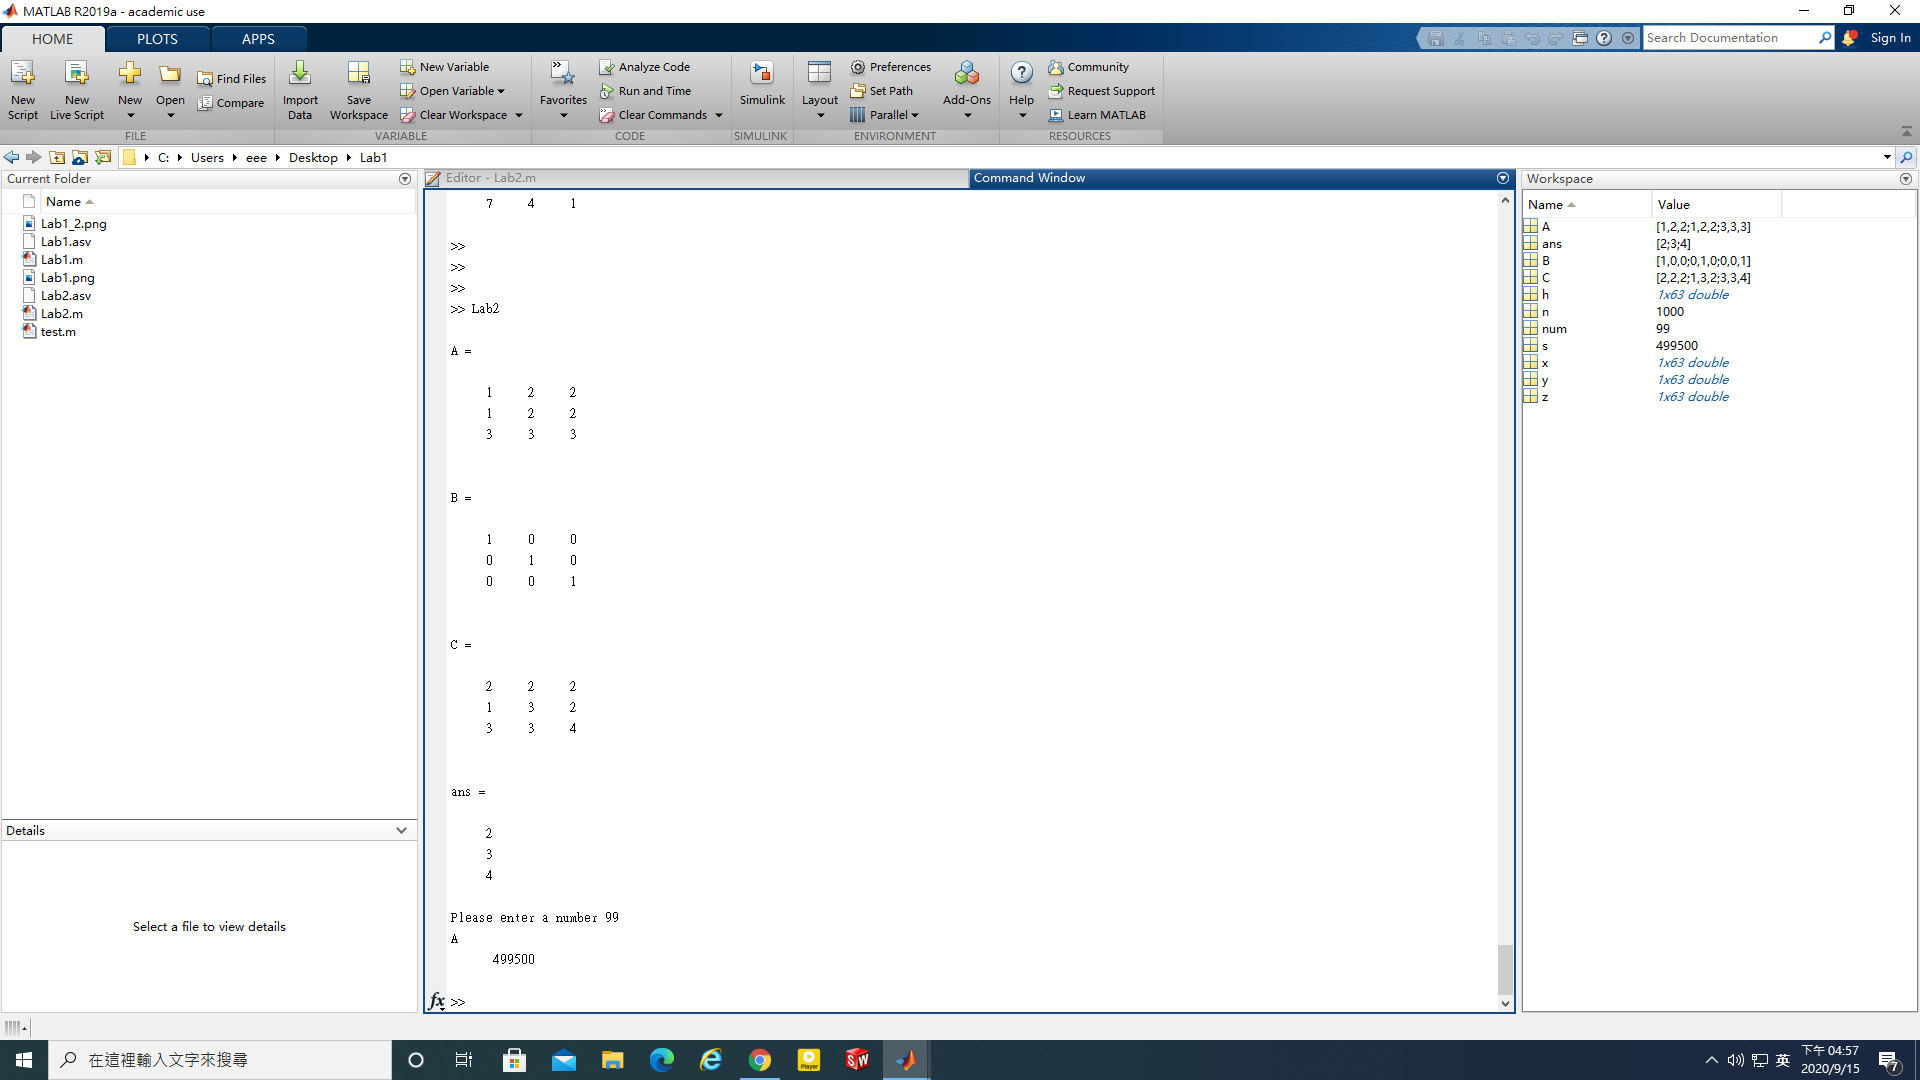
\includegraphics[scale=0.3]{HW first week 9_15 lab/Lab2/Lab2.png}

\section{Conclusion}
This is the first lab class in Matlab which is still easy for now, however, in order to perform well in Matlab coding, practices are needed. As a result, these basic operations should eventually become an instinct as a Matlab Programmer.Otherwise, future courses involving these kinds of basic operators might be difficult for those who did not practice well.And also this give me a chance to practice making report with Latex which is a pretty good tool for thesis writing.\\
\begin{center} 
This concludes the first Week Auto Control LAB\\
\end{center}

\end{document} 
